\addcontentsline{toc}{section}{Infinite non-linearity (2)}
\section*{Infinite non-linearity}

\begin{wrapfigure}{r}{.51\textwidth}
    \centering

    \begin{subfigure}[l]{.143\textwidth}
        \centering
        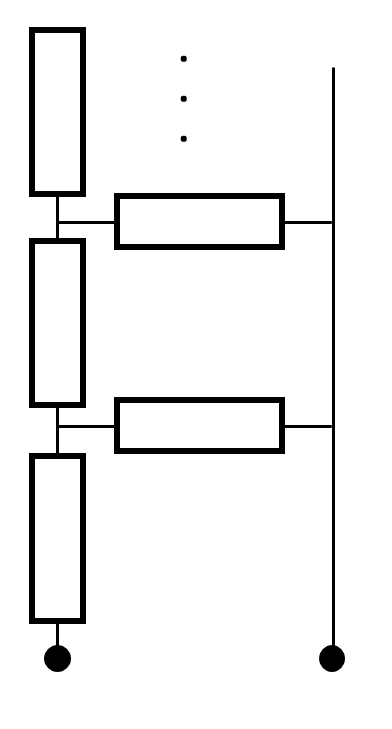
\includegraphics[width = \textwidth]{P-1}
        \caption{The system.}
        \labelf{P-1}
    \end{subfigure}
    \hfill
    \begin{subfigure}[l]{.3\textwidth}
        \centering
        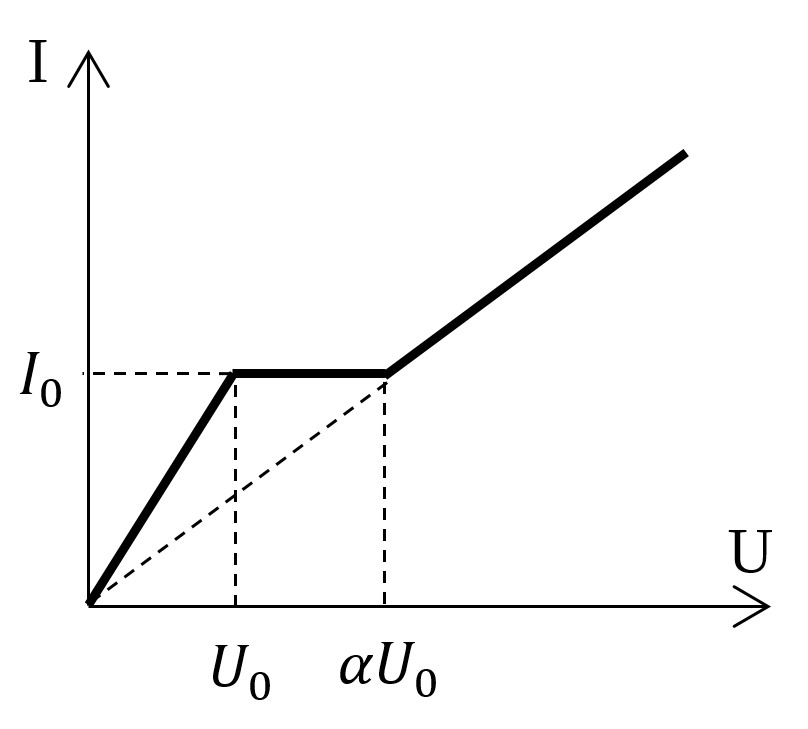
\includegraphics[width = \textwidth]{P-2}
        \caption{CVC of an element.}
        \labelf{P-2}
    \end{subfigure}
    
    \caption{}
    \labelf{P-1-2}
    \vspace{-1cm}
\end{wrapfigure}
\subsection*{Problem}

A system shown in \reff{P-1}
is composed of infinite number of identical non-linear elements.
The current-voltage characteristic (CVC) of an element in shown on \reff{P-2}. 
Qualitatively portray the CVC of the whole system.
Explicitly show 3 essential points on it (except $0-0$) and
describe the behavior for very big voltages.

\vspace{2cm}

\subsection*{Solution}

\begin{wrapfigure}{l}{.25\textwidth}
    \vspace{-.75cm}
    \centering
    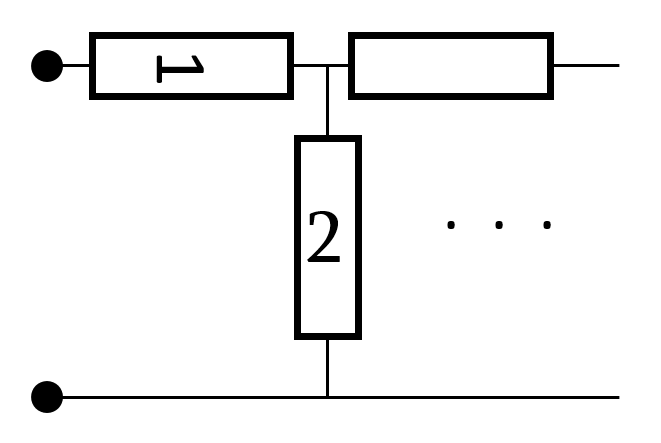
\includegraphics[width = .25\textwidth]{S-1}
    \caption{The system.}
    \labelf{S-1}
    \vspace{-.5cm}
\end{wrapfigure}

Let's gradually increase the voltage on the system.
It is obvious that
all the elements will be in their first linear domain in the beginning.
In this case every element behaves like a simple resistor
with resistance $R_0 = U_0 / I_0$.
In this case the overall resistance $R$ will be given by infamous relation
\begin{equation}
    \frac{R R_0}{R + R_0} + R_0 = R
\end{equation}
from which we get
\begin{equation}
    R = R_0 \frac{1+\sqrt{5}}{2}
\end{equation}

This will continue until one of the elements
gets out of its linear region.
Obviously it will be the one with the biggest current,
indexed as $1$ in \reff{S-1}.
It will reach current $I_0$ when $U = I_0 R$ and stabilize
as shown on \reff{S-2}.

\begin{wrapfigure}{r}{.5\textwidth}
    \centering
    \vspace{-.5cm}
    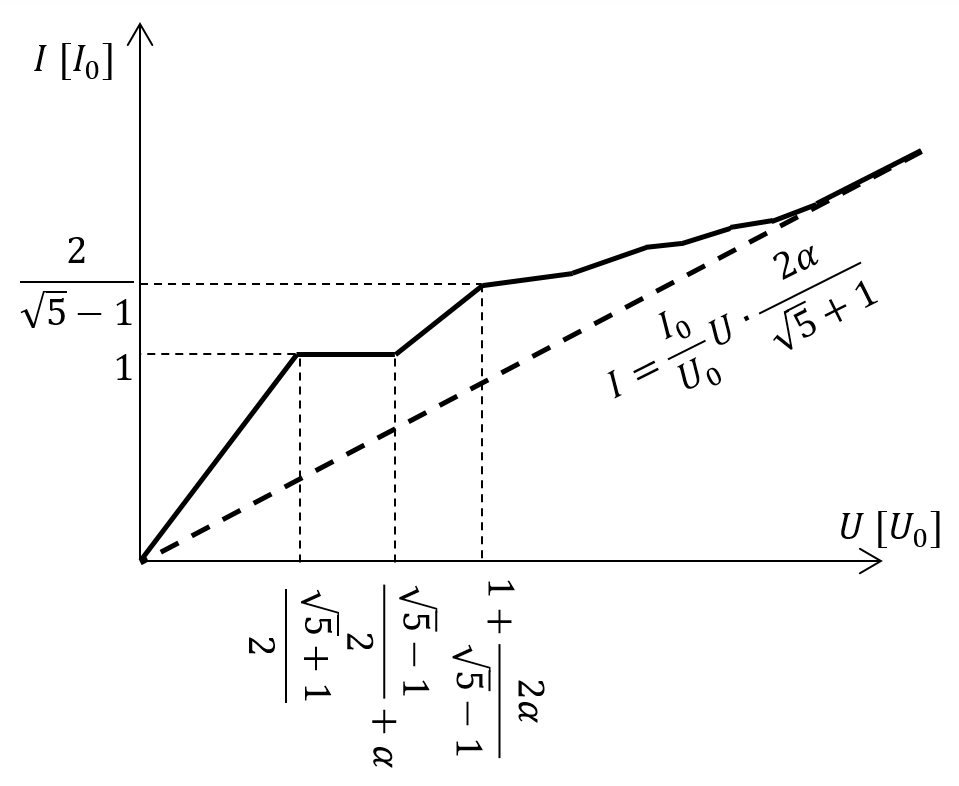
\includegraphics[width = .5\textwidth]{S-2}
    \caption{CVC of the whole system.}
    \labelf{S-2}
    \vspace{-.5cm}
\end{wrapfigure}

In order to have bigger current in the system,
the element $1$ should leave its constancy domain.
until then the state of the other element doesn't change
and all the additional voltage falls on $1$.
When the later's voltage is $\alpha U_0$,
the voltage on the whole system is $\alpha U_0 + I_0 (R - R_0)$.
It's the second breaking point on \reff{S-2}.
Element $1$ behaves like a resistor with resistance $\alpha R_0$ afterwards.

The next element to leave its first linear domain is $2$ \reff{S-1}
as it has the highest voltage of the remaining elements.
It is straightforward to calculate the current and the voltage of the system
when the voltage on $2$ is $U_0$.
The answer is depicted of \reff{S-2} as the third breaking point.

For big enough values of voltage
all the elements will be in their second linear domain
and the system will have resistance $\alpha R_0 (1+\sqrt{5})/2$
